\section{}
A rectangular plate is subjected to uniform tensile stress $\sigma$ along its upper and 
lower edges as shown in Fig. \ref{fig:Q3}. Determine the displacements $u$ and $v$ in terms 
of $x$, $y$, and material properties ($E$, $\nu$) using Eqns. (\ref{eq:Q3Strain}) and (\ref{eq:Q3Shear}) and the appropriate 
conditions at the origin.

\begin{figure}[h]
    \centering
    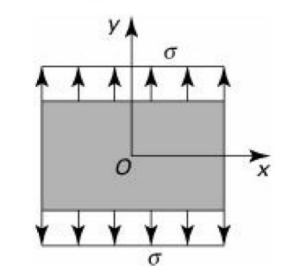
\includegraphics[width=0.3\linewidth]{Questions/Figures/Q3ProblemDiagram.png}
    \caption{Rectangular plate subjected to uniform tensile stress.}
    \label{fig:Q3}
\end{figure}

\begin{align}
    \epsilon_x &= \frac{\partial u}{\partial x}, \;\; \epsilon_y = \frac{\partial v}{\partial y} \label{eq:Q3Strain} \\
    \gamma_{xy} &= \alpha_x - \alpha_y = \frac{\partial u}{\partial y} + \frac{\partial v}{\partial x} \label{eq:Q3Shear}
\end{align}

\textbf{Solution}
\subsection{}

First we derive expressions for $\epsilon_x$ and $\epsilon_y$ in terms of $E$, $\nu$, and $\sigma$. By generalized Hooke's law,
\[
\begin{aligned}
    \epsilon_x &= \frac{1}{E} (\cancel{\sigma_x} - \nu(\sigma_y))
    &= \frac{-\nu\sigma_y}{E} \\
    \epsilon_y &= \frac{1}{E} (\sigma_y- \nu( \cancel{\sigma_x}))
    &= \frac{\sigma_y}{E} \\
\end{aligned}
\]

By direct substitution,
\[
\begin{aligned}
    \epsilon_x &= \frac{-\nu\sigma}{E} = \frac{\partial u}{\partial x} \\
    \epsilon_y &= \frac{\sigma}{E} = \frac{\partial v}{\partial y} \\
\end{aligned}
\]

Integrating,
\[
\begin{aligned}
    \int \partial u &= \int \frac{-\nu\sigma}{E} \partial x \\
    u &= \frac{-\nu\sigma}{E} x + g(y) \\
    \int \partial v &= \int \frac{\sigma}{E} \partial y \\
    v &= \frac{\sigma}{E} y + h(x) \\
\end{aligned}
\]

Where $g(y)$ and $h(x)$ are arbitrary functions of $y$ and $x$, respectively. We can determine the functions $g(y)$ and $h(x)$ 
by applying the boundary conditions. Define the origin such that ($x, y$) = (0, 0), ($u, v$) = (0, 0). As a consequence, 
shear strain $\gamma_{xy}$ is zero at the origin. By Eqn. (\ref{eq:Q3Shear}),
\[
\begin{aligned}
    \gamma_{xy} &= \frac{\partial u}{\partial y} + \frac{\partial v}{\partial x} \\
    0 &= \frac{\partial}{\partial y} \left(\frac{-\nu\sigma}{E} x + g(y)\right) + \frac{\partial}{\partial x} 
    \left(\frac{\sigma}{E} y + h(x)\right) \\
    0 &= g'(y) + h'(x) \\
    g'(y) &= -h'(x) = -\lambda \\
\end{aligned}
\]

Where $\lambda$ is a constant. Integrating gives us $g(y) = c_1$ and $h(x) = c_2$. By the boundary conditions, ($u, v$) = (0, 0) at ($x, y$) = (0, 0).
\[
\begin{aligned}
    u|_{(0, 0)} &= \frac{-\nu\sigma}{E} (0) + c_1 \overset{\text{set}}{=} 0 \\
    \implies c_1 &= 0 \\
    v|_{(0, 0)} &= \frac{\sigma}{E} (0) + c_2 \overset{\text{set}}{=} 0 \\
    \implies c_2 &= 0 \\
\end{aligned}
\]

Therefore, the final expressions for $u$ and $v$ are given by:
\begin{empheq}[box = \fbox]{align*}
    u &= \frac{-\nu\sigma}{E} x \\
    v &= \frac{\sigma}{E} y 
\end{empheq}